\documentclass{standalone}

\usepackage{bm}
\usepackage{tikz}

\begin{document}
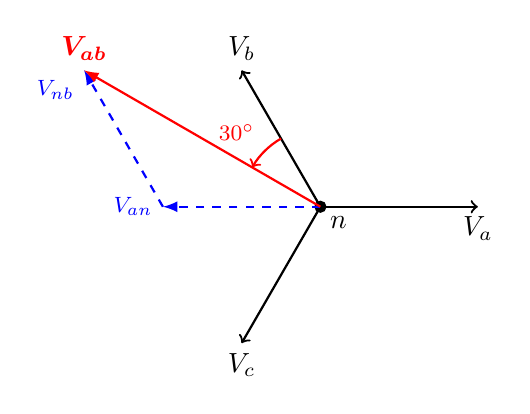
\begin{tikzpicture}
    % Define the three phase voltages
    \draw[->, thick] (0,0) -- (2,0) node[anchor=north] {$V_a$};
    \draw[->, thick] (0,0) -- (-1,1.732) node[anchor=south] {$V_b$};
    \draw[->, thick] (0,0) -- (-1,-1.732) node[anchor=north] {$V_c$};
    
    % Draw the neutral point
    \filldraw[black] (0,0) circle (2pt) node[anchor=north west] {$n$};

    % Draw V_ab in red, V_an in dashed red
    \draw[-latex, thick, dashed, blue] (0,0) -- (-2,0) node[anchor=east] {\footnotesize $V_{an}$};
    \draw[-latex, thick, dashed, blue] (-2,0) -- (-3,1.732) node[anchor=north east] {\footnotesize $V_{nb}$};
    \draw[-latex, thick, red] (0,0) -- (-3,1.732) node[anchor=south] {$\bm{V_{ab}}$};

    % Angle (from V_b to V_ab)
    \draw[->, thick, red] (-0.5,0.866) arc (120:150:1) node[midway, anchor=south east] {\footnotesize $30^\circ$};
\end{tikzpicture}
\end{document}